\documentclass[10pt]{article}
\usepackage{amsmath,amssymb}
\setlength{\oddsidemargin}{0in}
\setlength{\evensidemargin}{0in}
\setlength{\textheight}{9in}
\setlength{\textwidth}{6.5in}
\setlength{\topmargin}{-0.5in}
\usepackage{enumitem}
\usepackage{graphicx}
\usepackage{float}

\title{\bf Math 170S: Homework 1}
\date{10/13/2023}
\author{\bf Owen Jones}

\begin{document}
\maketitle
\begin{enumerate}[label=\textbf{Problem \arabic*.}]
    \item \begin{itemize}
        \item [1.] $\overline{x}=7.2333,s^2=4.1823,s=2.0451$
        \item [2.] within one std: $24$, within two std: $29$
    \end{itemize}
    \item $\overline{y}=\frac{\displaystyle\sum_{i=1}^{n}y_i}{n}=\frac{\displaystyle\sum_{i=1}^{n}ax_i+b}{n}=\frac{\displaystyle nb+a\sum_{i=1}^{n}x_i}{n}=a\frac{\displaystyle\sum_{i=1}^{n}x_1}{n}+b=a\overline{x}+b$\\
    $s_y^2=\frac{\displaystyle \sum_{i=1}^{n}{(y_i-\overline{y})}^2}{n-1}=\frac{\displaystyle \sum_{i=1}^{n}{(ax_i+b-(a\overline{x}+b))}^2}{n-1}=\frac{\displaystyle a^2\sum_{i=1}^{n}{(x_i-\overline{x})}^2}{n-1}=a^2s_x^2$
    \item \begin{itemize}
        \item [1.] $\pi_{25}=6.0,\pi_{75}=8.25,IQR=2.25$
        \item [2.] $\pi_{10}=5.18,\pi_{90}=9.34$
        \item [3.] suspected outliers: $14.1$
    \end{itemize}
    \item \begin{itemize}
        \item [1.] $P(Y_7<27.3)=\displaystyle\sum_{k=7}^{8}\begin{pmatrix}
            8\\
            k
        \end{pmatrix} {(0.7)}^k{(0.3)}^{8-k}=0.2553$
        \item [2.]  $P(Y_5<27.3<Y_8)=\displaystyle\sum_{k=5}^{7}\begin{pmatrix}
            8\\
            k
        \end{pmatrix} {(0.7)}^k{(0.3)}^{8-k}=0.7482$
    \end{itemize}
    \begin{figure}[H]
        \centering
        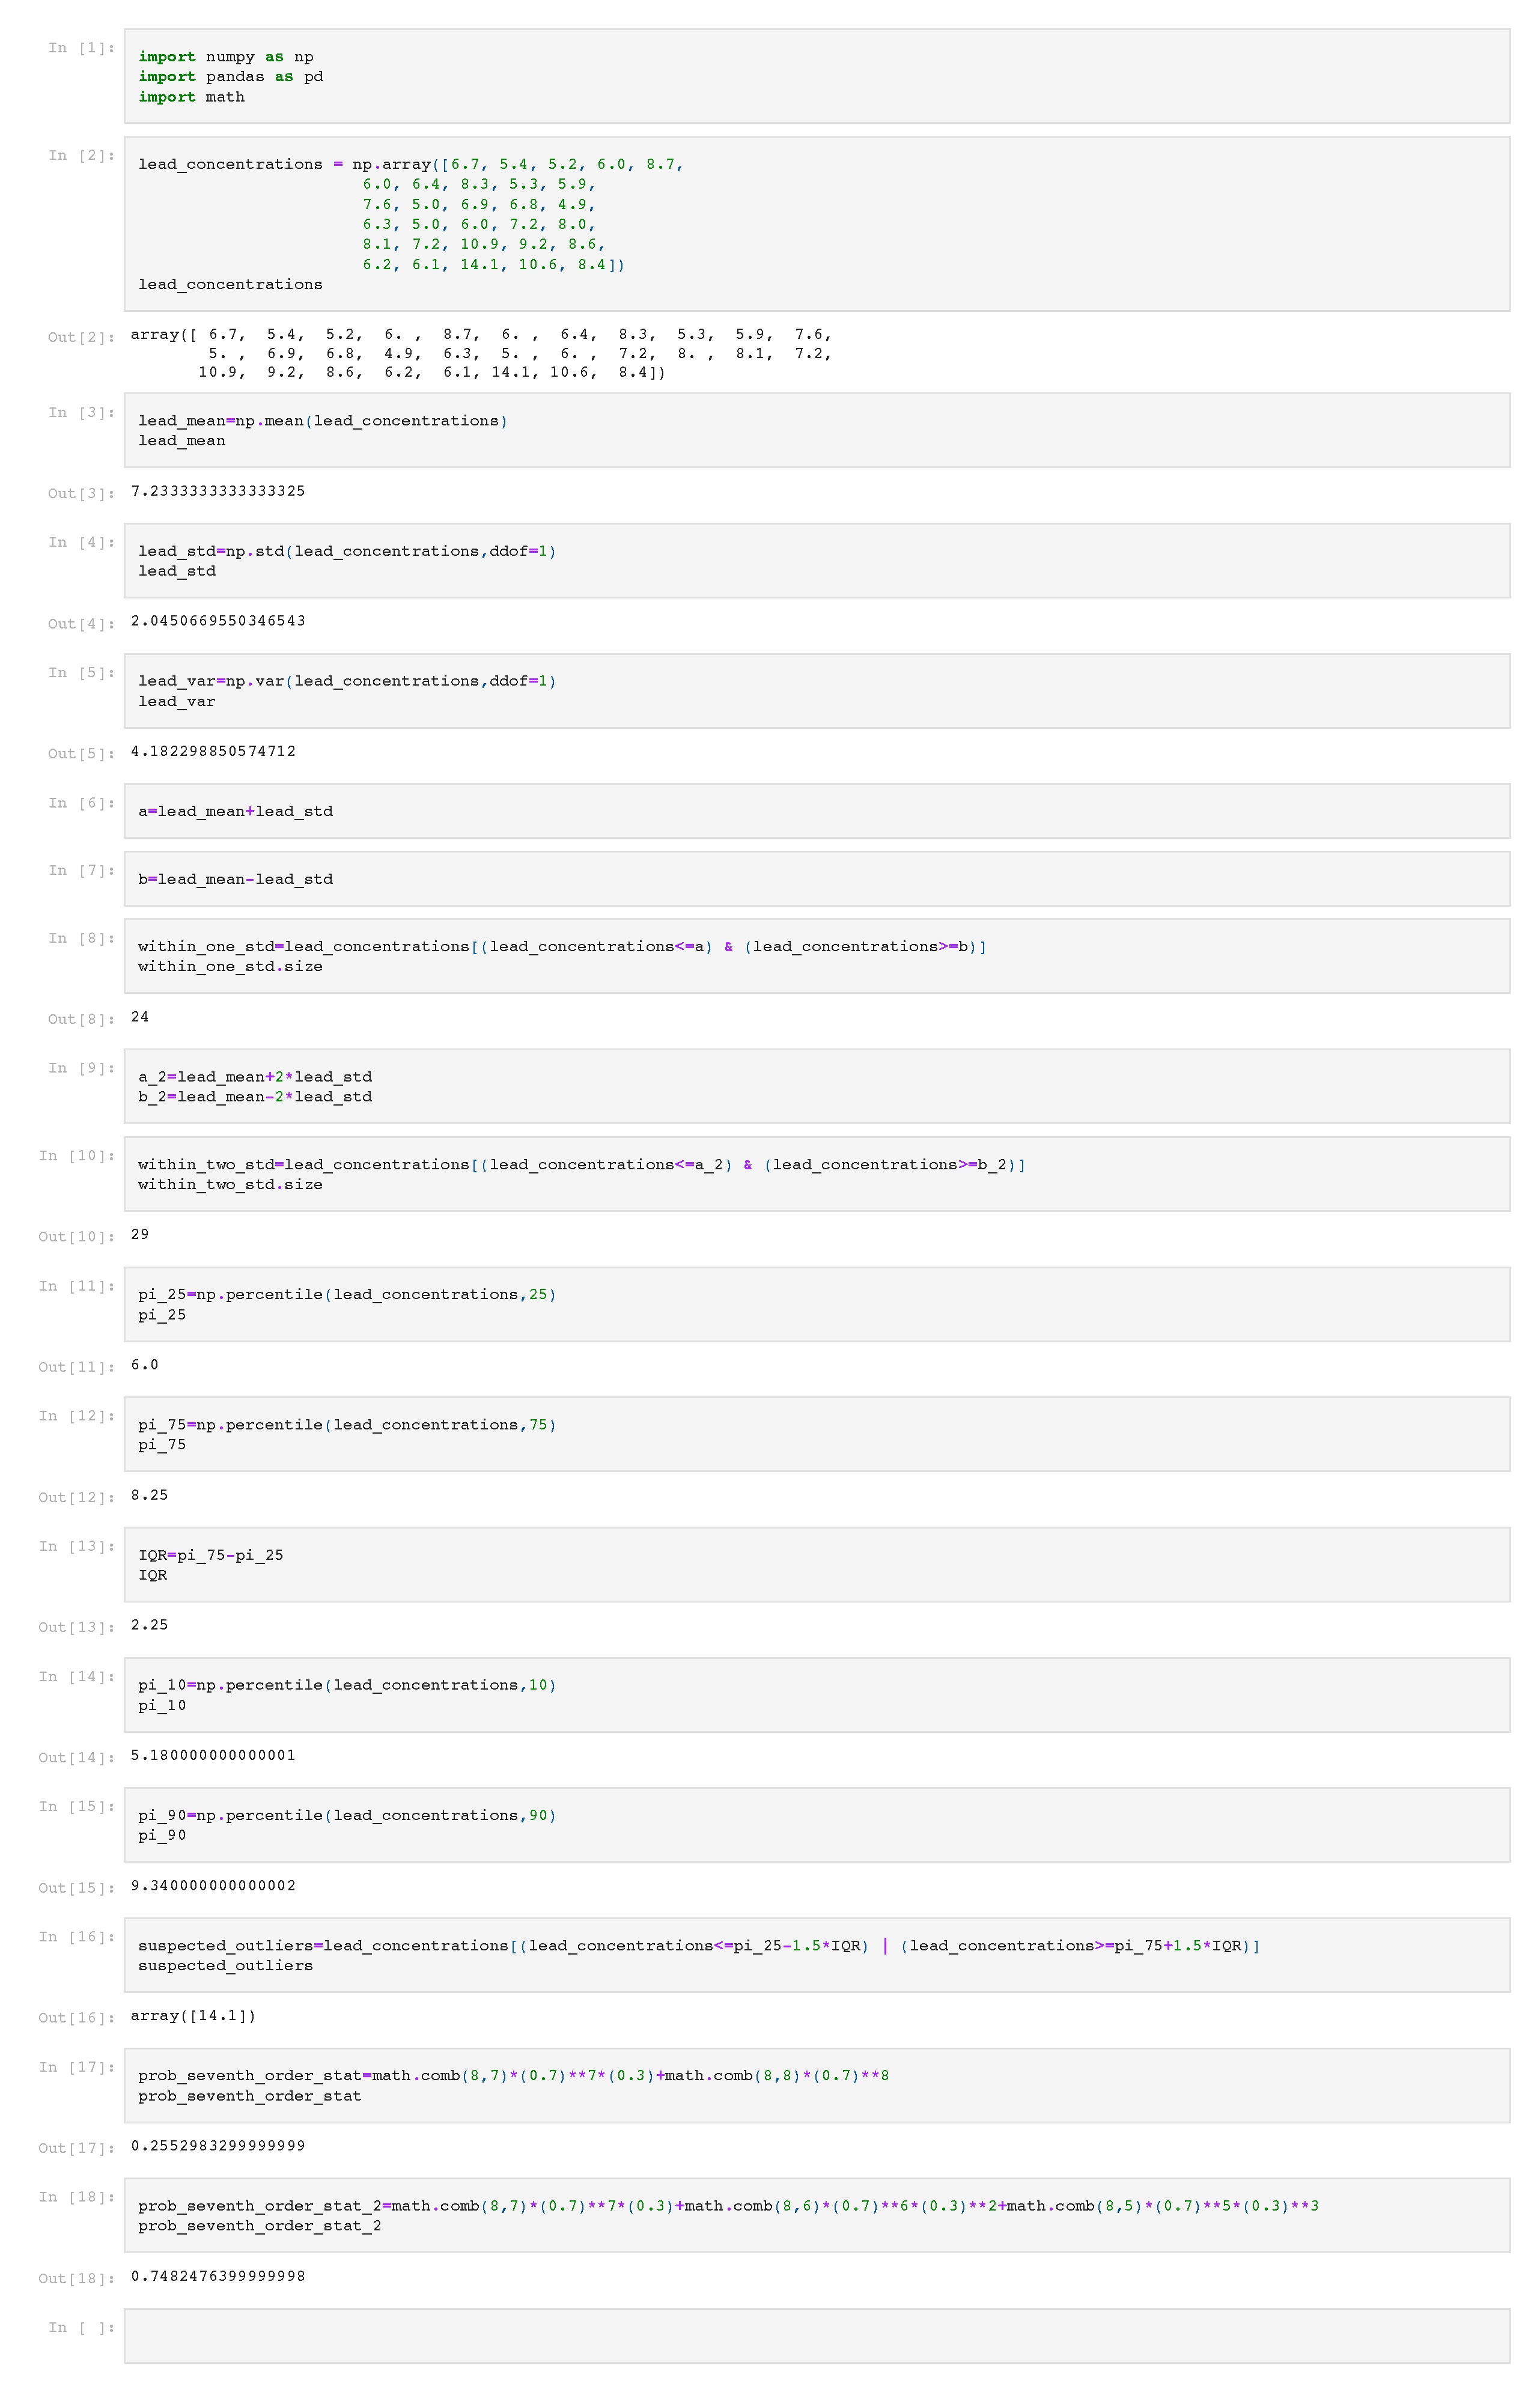
\includegraphics[scale=0.2]{Math_170S_Homework_1_jupyter.pdf}
    \end{figure}
    \item \begin{itemize}
        \item [1.] $\displaystyle E[W_r^2]=\int_{0}^{1}w^2g_r(w)dw\\
        =\int_{0}^{1}w^2\frac{n!}{(r-1)!(n-r)!}{[w]}^{r-1}{[1-w]}^{n-r} dw\\
        =\frac{r(r+1)}{(n+1)(n+2)}\int_{0}^{1}\frac{(n+2)!}{(r+1)!(n-r)!}{[w]}^{r+1}{[1-w]}^{n-r} dw\\
        =\frac{r(r+1)}{(n+1)(n+2)}\int_{0}^{1}Beta(r+2,n-r+1) dw\\
        =\frac{r(r+1)}{(n+1)(n+2)}\cdot1$
        \item [2.] $Var[W_r]=E[W_r^2]-{E[W_r]}^2=\frac{r(r+1)}{(n+1)(n+2)}-\frac{r^2}{{(n+1)}^2}=\frac{r(r+1)(n+1)}{{(n+1)}^2(n+2)}-\frac{r^2(n+2)}{{(n+1)}^2(n+2)}=\frac{r(n-r+1)}{{(n+1)}^2(n+2)}$
    \end{itemize}
\end{enumerate}
\end{document}